\section{Experimento 1}


En este experimento, observaremos el funcionamiento de una máquina de tracción-compresión, llamada Maquina Universal de Ensayo.

\subsection{Sensores que utiliza}

Los sensores que utiliza la máquina son:\\

En la primera y segunda imagen se puede observar un transductor de desplazamiento lineal potenciométrico con punta de bola y resorte de retorno, se utiliza para medir el desplazamiento de la máquina.\\

En la tercera, cuarta y quinta imagen se observa un transmisor o sensor de presión hidráulica, la fuerza que se aplica a la probeta es transmitida a través de un fluido hidráulico, y este sensor mide la presión que ejerce el fluido.\\

La sexta imagen corresponde a una unidad de potencia hidráulica, que es el motor eléctrico conectado a la bomba hidráulica, además se puede observar a la derecha el filtro hidráulico con un indicador visual de saturación.

La ultima imagen corresponde a una servoválvula que es el conjunto de electroválvulas y servoválvula hidráulica que controla el caudal y la dirección del fluido hidráulico hacia el actuador con gran precisión.


\subsection{Procedimiento y Datos}

Durante el experimento se puso en marcha la máquina de tracción-compresión, y se aplicó una fuerza a la probeta hasta su punto de ruptura.\\

Alguno de los datos obtenidos durante el experimento fueron:\\

\begin{itemize}
	\item Peso ejercido por la mpaquina por unidad de longitud: 15kg/m
	\item Logitud de estiramiento de la probeta: 12mm
	\item Peso de ruptura de la probeta: 4200kg
\end{itemize}

\subsection{Imagenes}

\begin{figure}[H]
	\centering
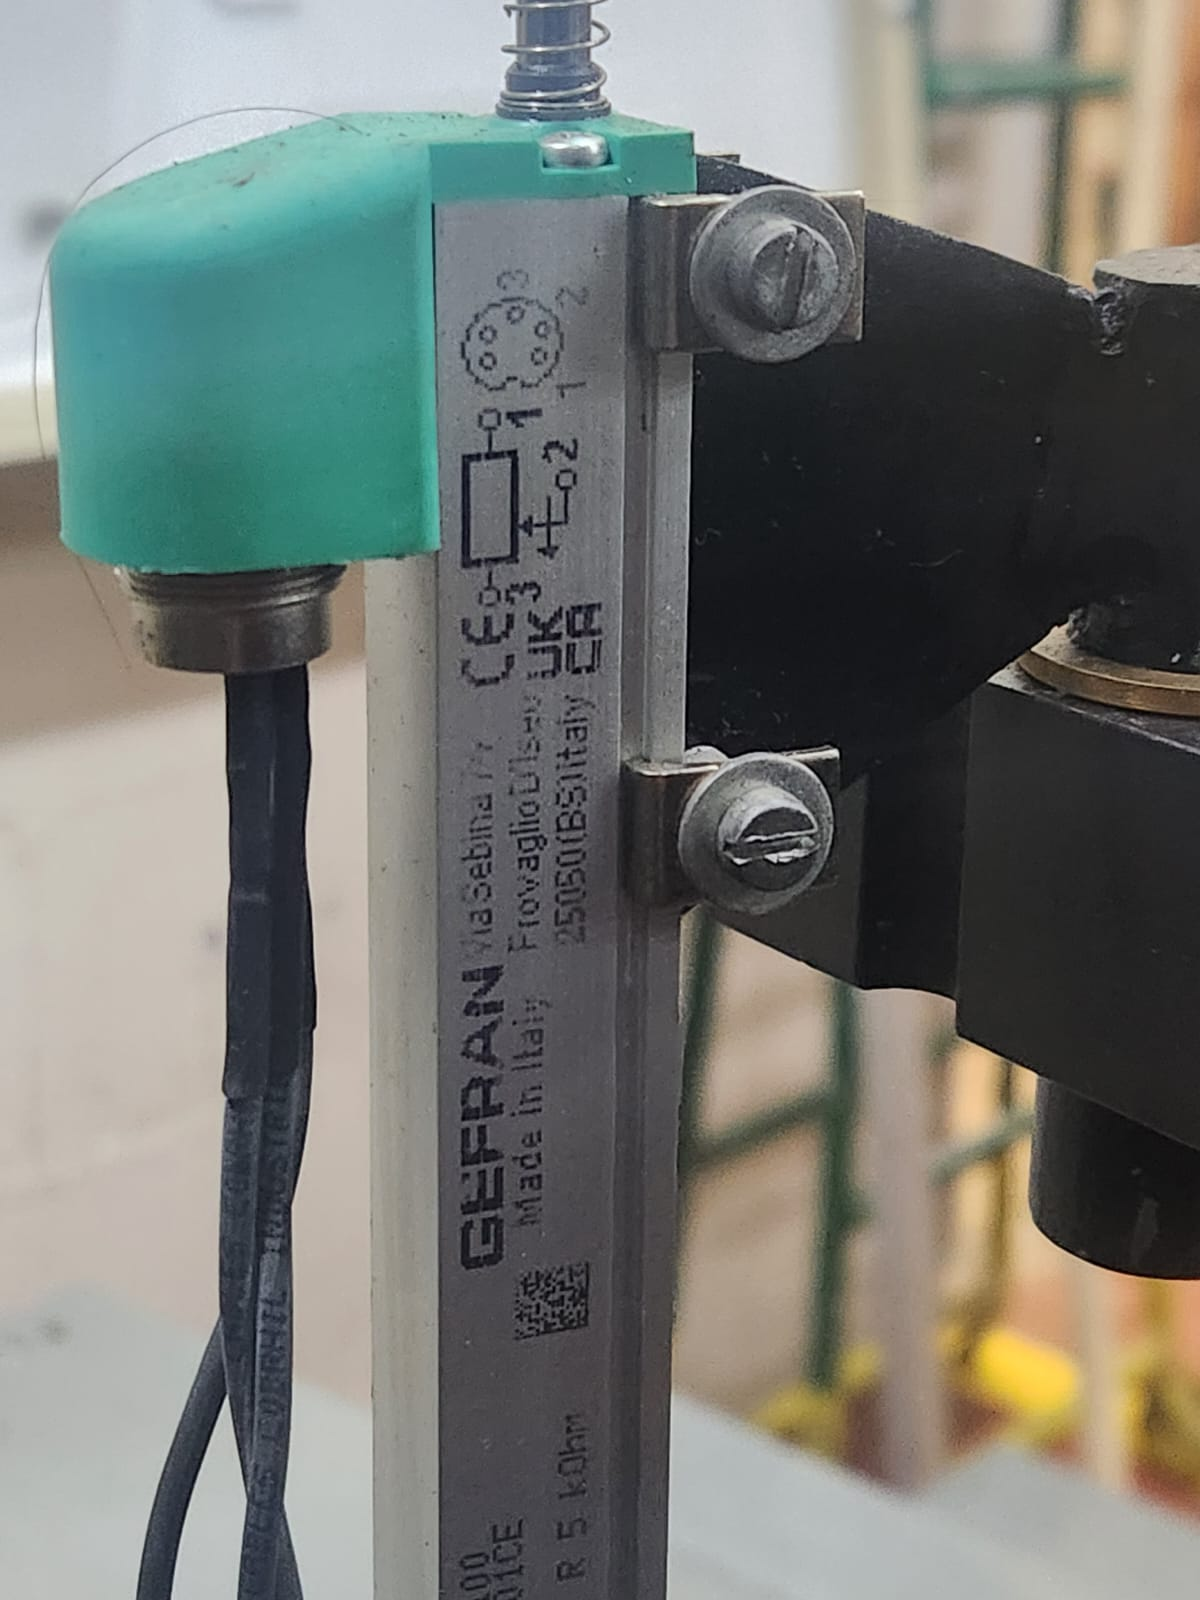
\includegraphics[width=0.3\textwidth]{images/1}
\caption{Imagen 1 de la máquina universal de ensayo.}
\end{figure}

\begin{figure}[H]
	\centering
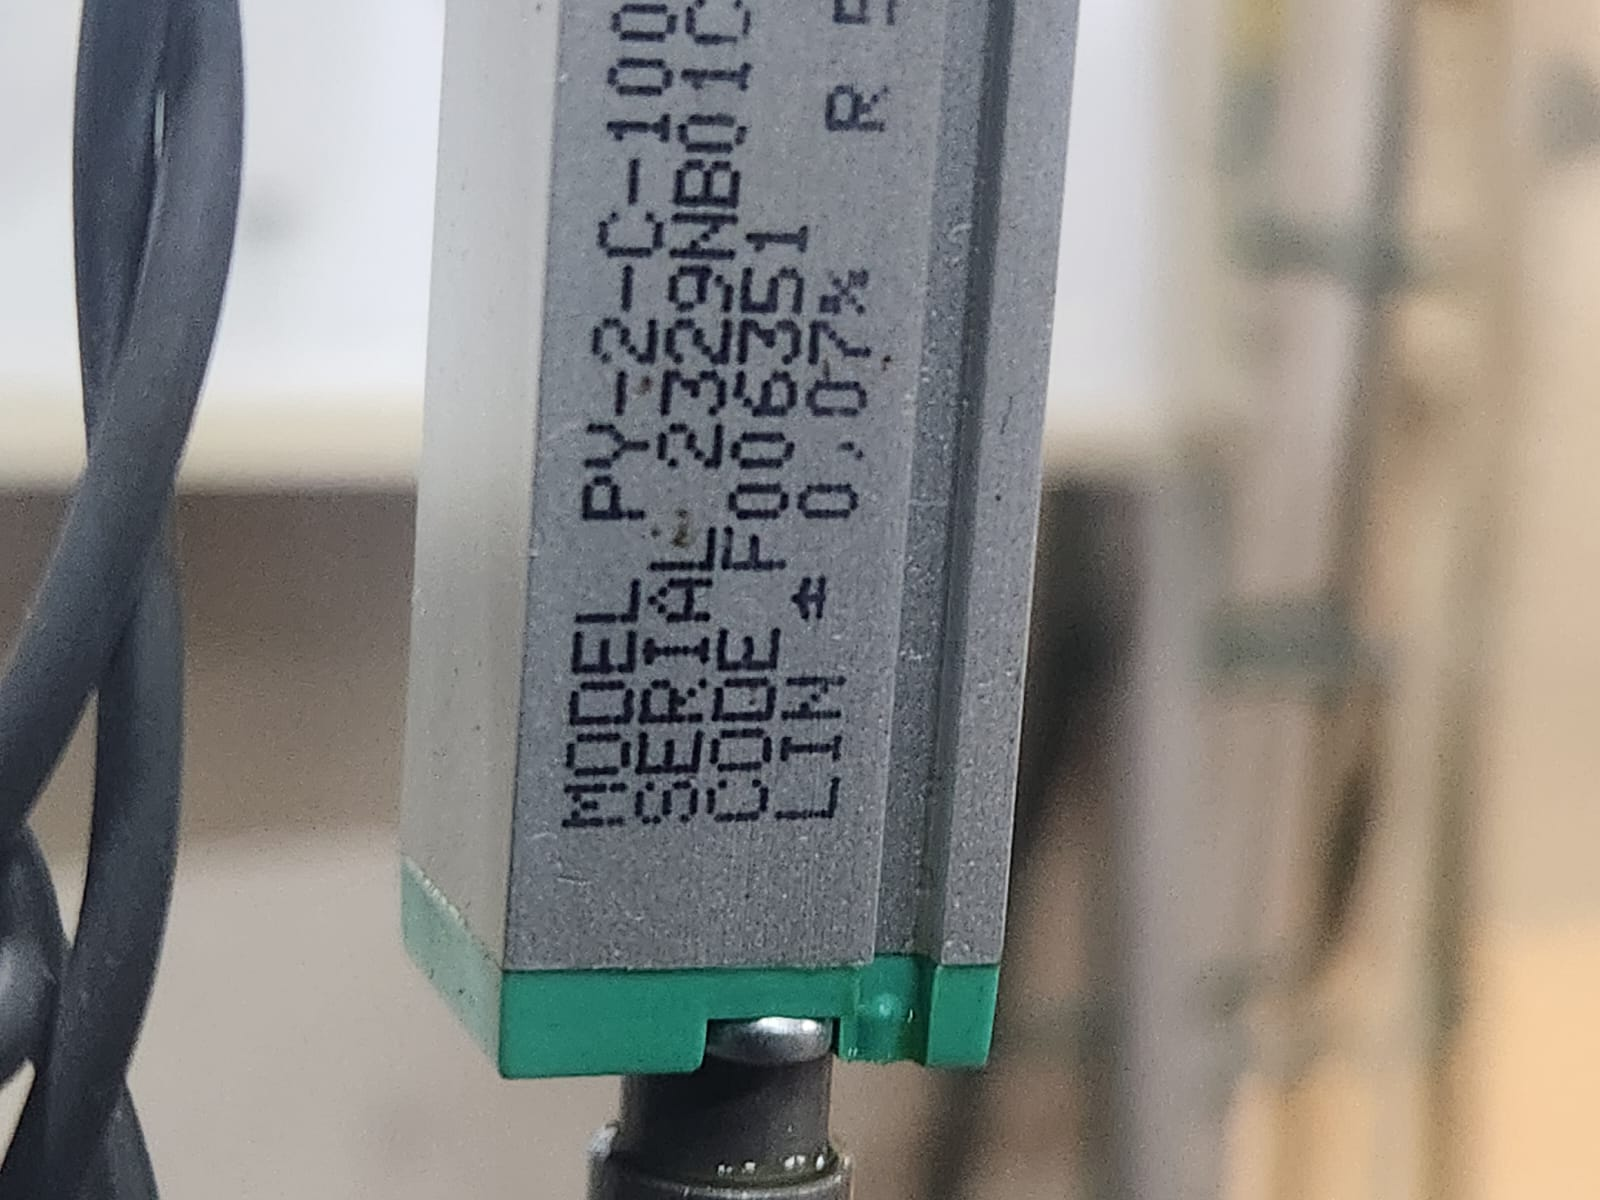
\includegraphics[width=0.3\textwidth]{images/2}
\caption{Imagen 2 de la máquina universal de ensayo.}
\end{figure}

\begin{figure}[H]
	\centering
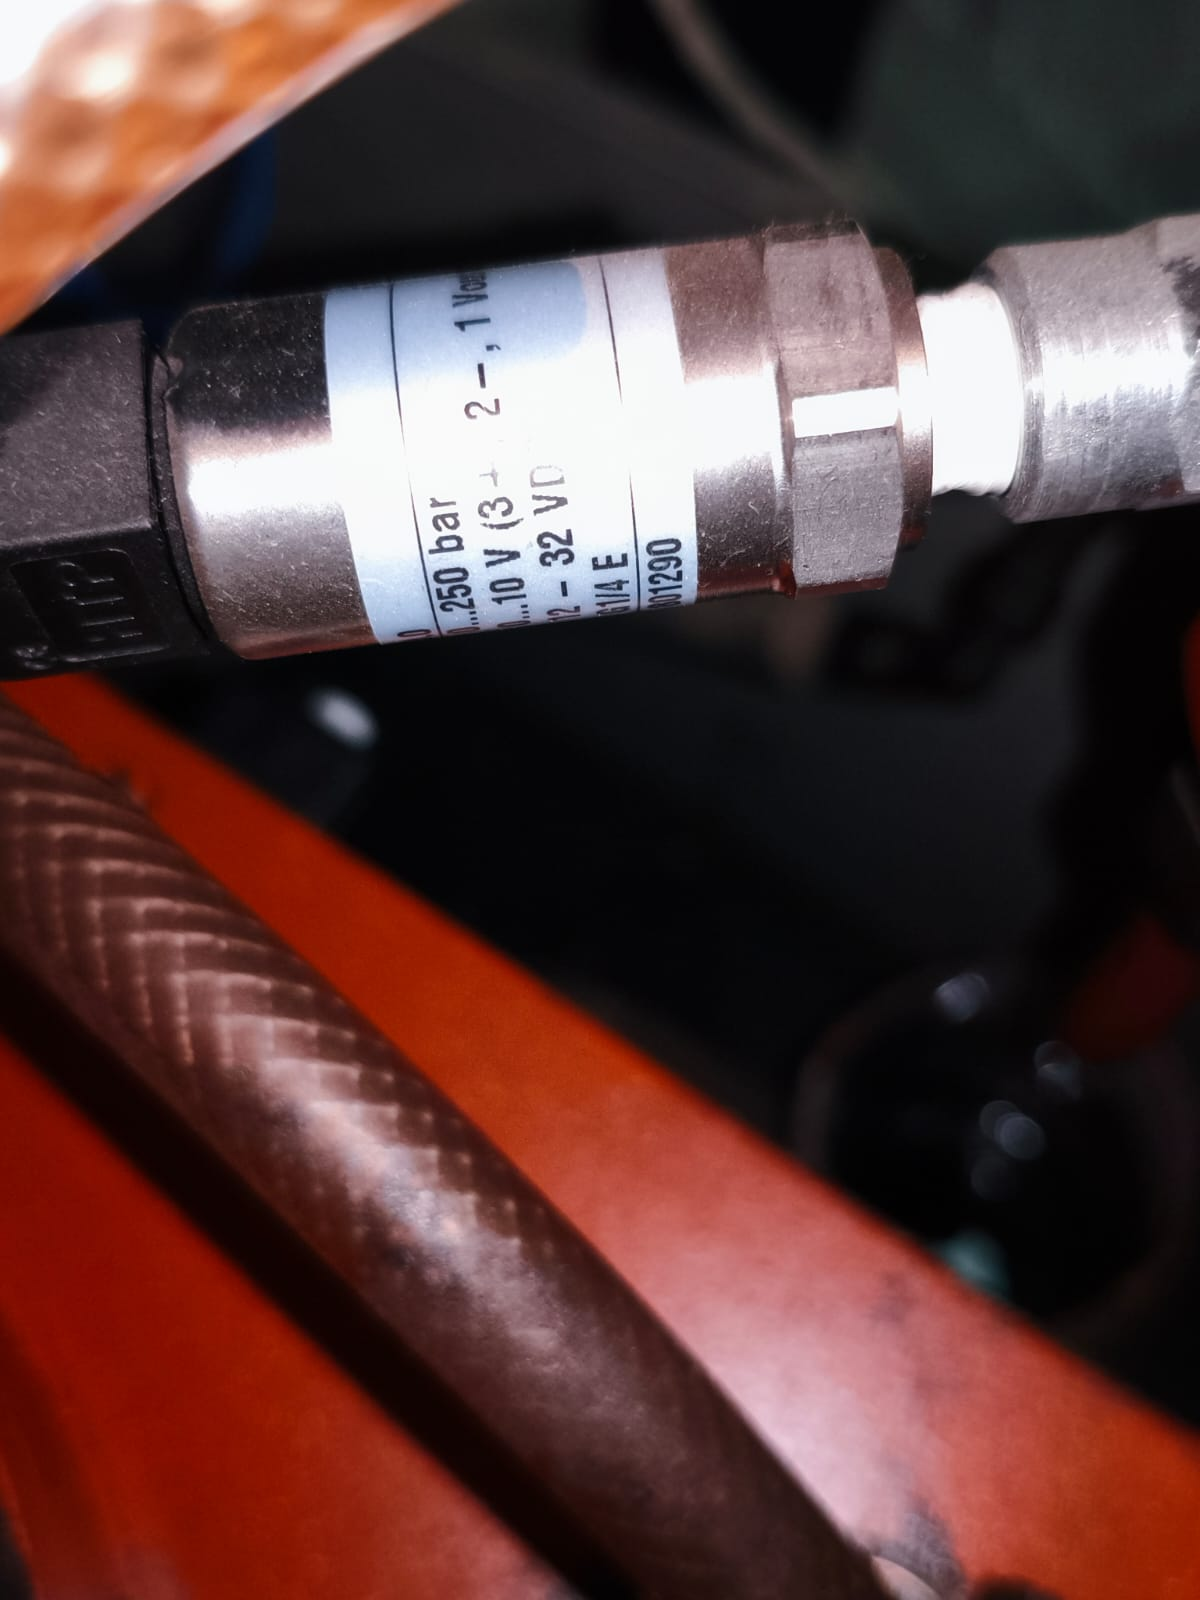
\includegraphics[width=0.3\textwidth]{images/4}
\caption{Imagen 3 de la máquina universal de ensayo.}
\end{figure}

\begin{figure}[H]
	\centering
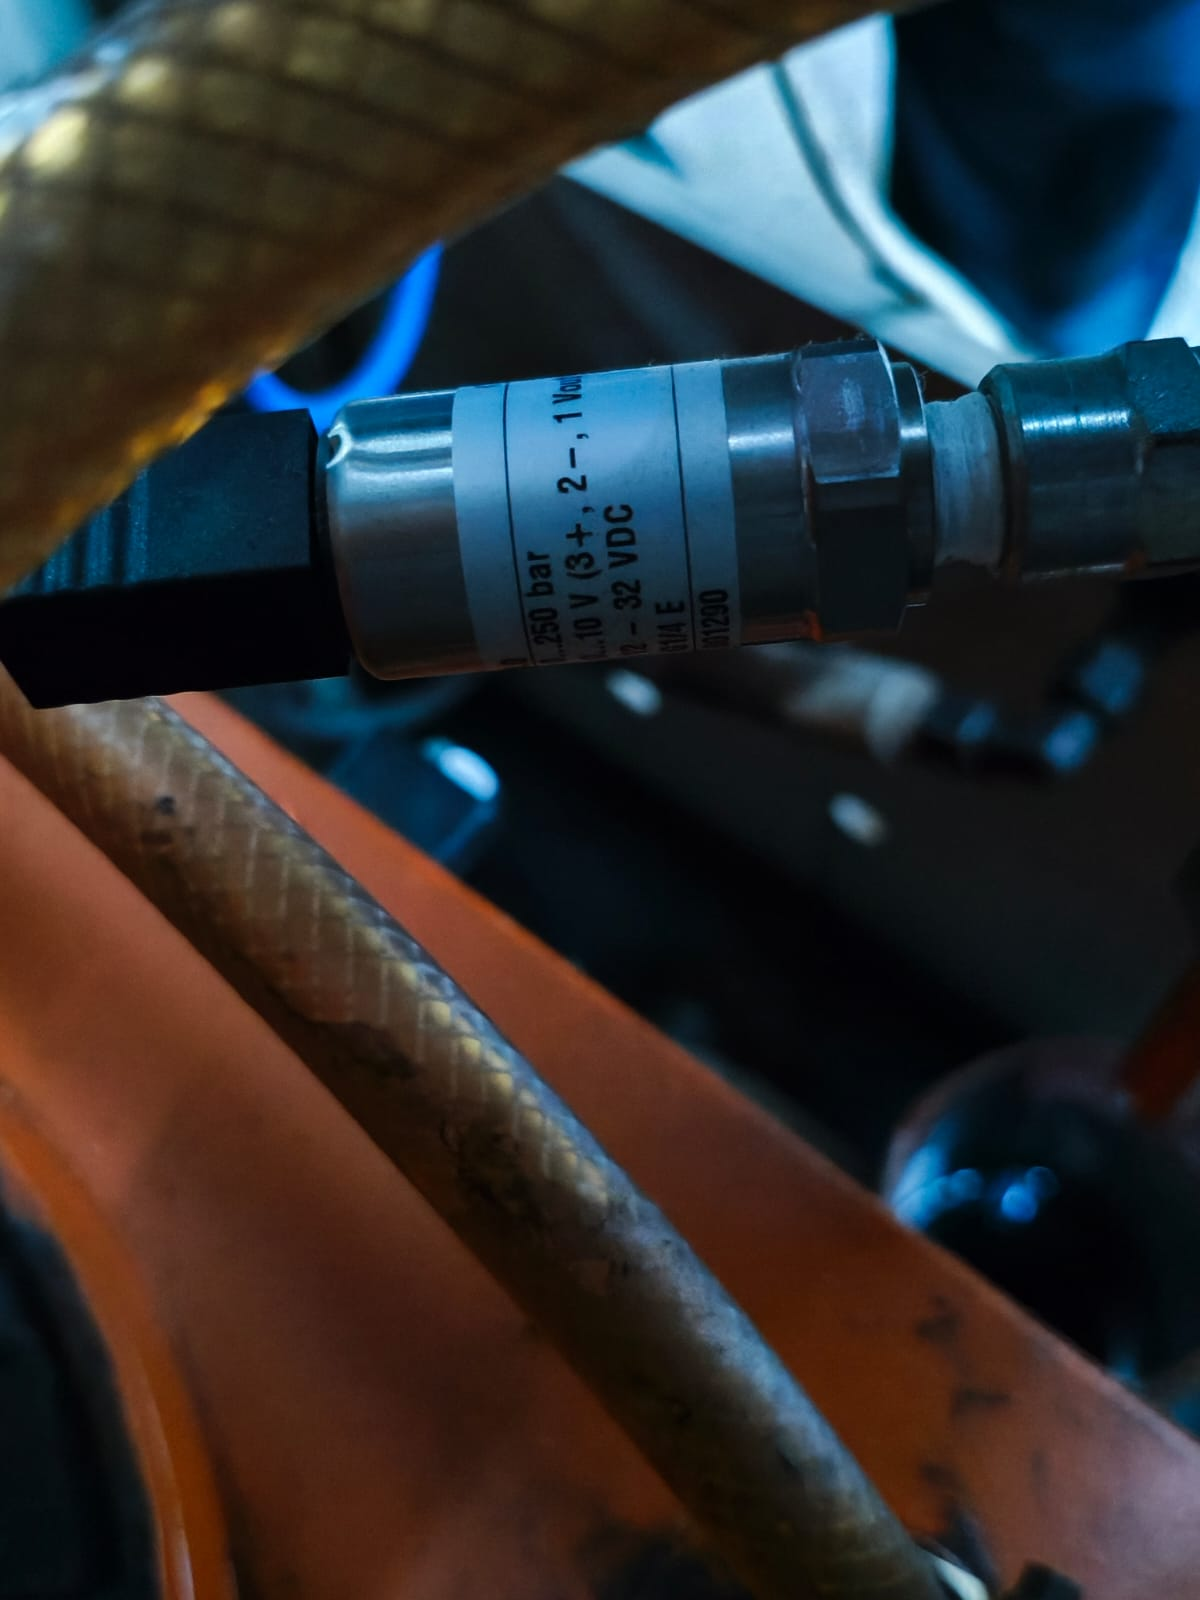
\includegraphics[width=0.28\textwidth]{images/6}
\caption{Imagen 4 de la máquina universal de ensayo.}
\end{figure}

\begin{figure}[H]
	\centering
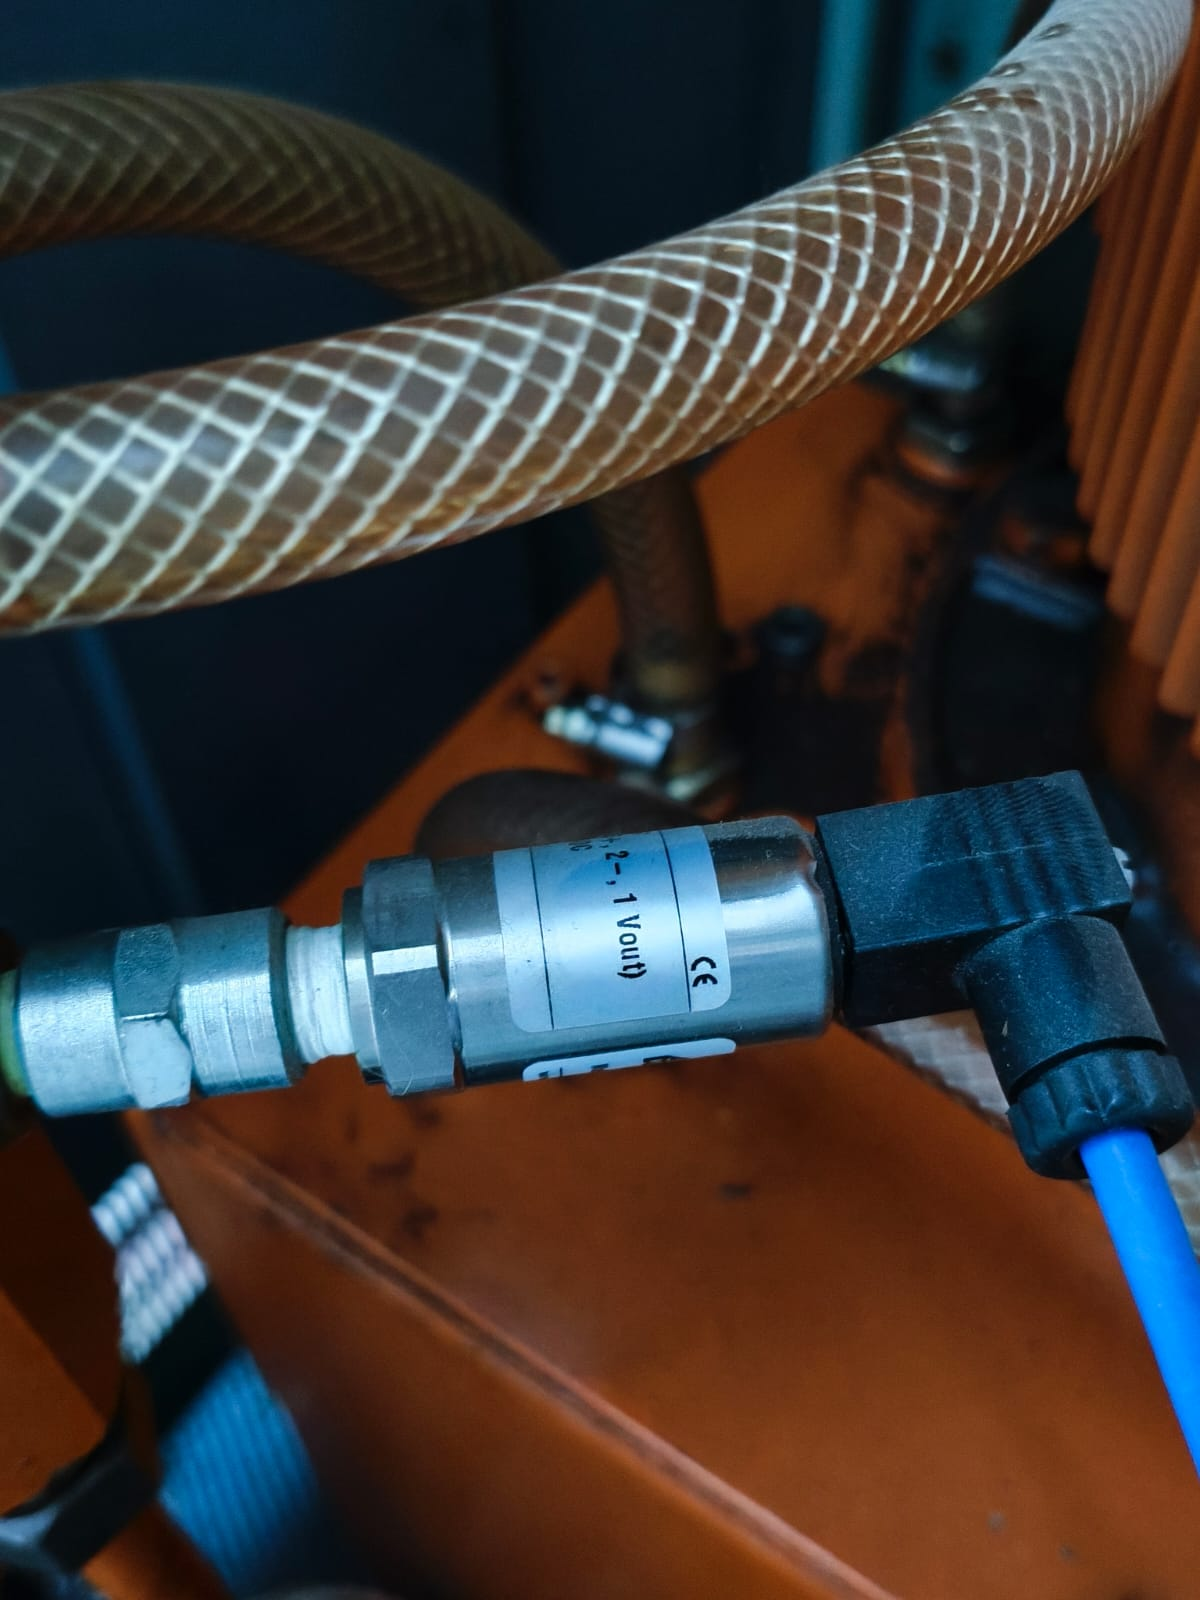
\includegraphics[width=0.3\textwidth]{images/7}
\caption{Imagen 5 de la máquina universal de ensayo.}
\end{figure}

\begin{figure}[H]
	\centering
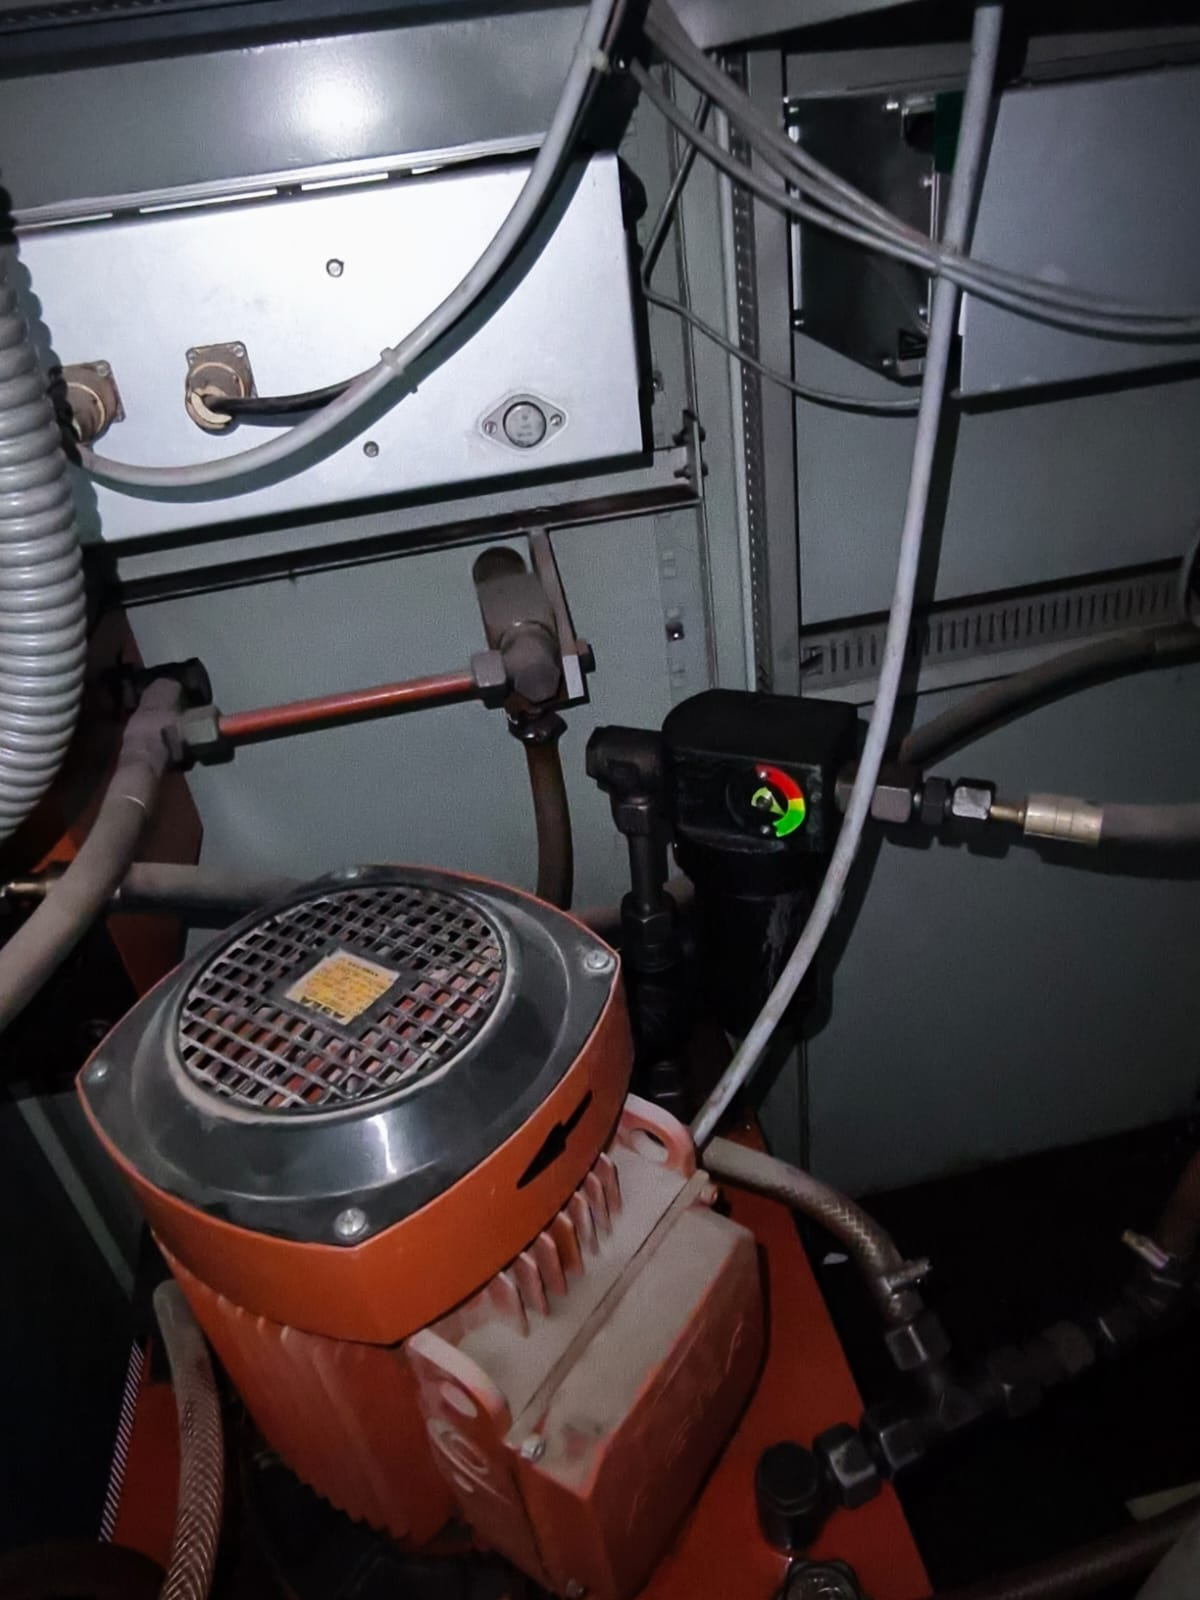
\includegraphics[width=0.3\textwidth]{images/5}
\caption{Imagen 6 de la máquina universal de ensayo.}
\end{figure}

\begin{figure}[H]
	\centering
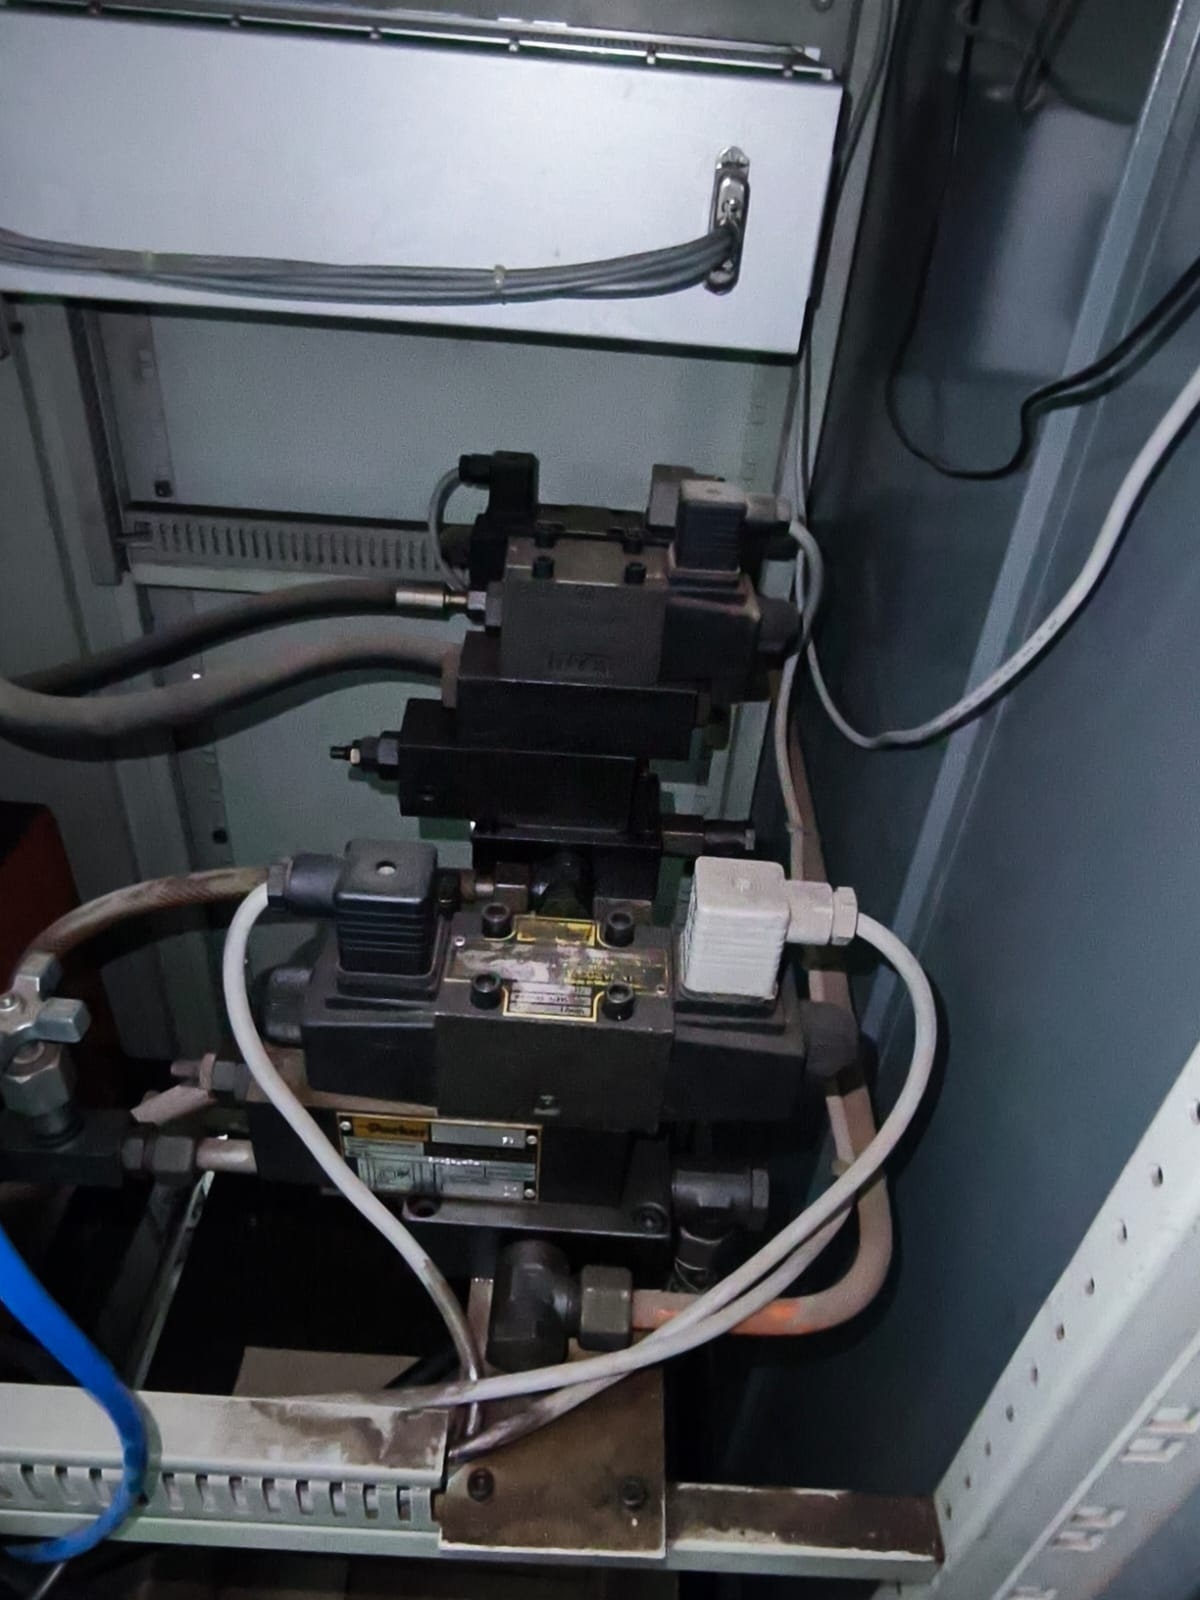
\includegraphics[width=0.3\textwidth]{images/8}
\caption{Imagen 7 de la máquina universal de ensayo.}
\end{figure}
